\documentclass[10pt]{beamer}
\usepackage[utf8]{inputenc}
\usepackage[francais]{babel}
\usepackage[T1]{fontenc}
\usepackage[export]{adjustbox}
\newcommand\Fontvi{\fontsize{8}{7.2}\selectfont}

\usepackage{minted}
\usemintedstyle{colorful}
\usepackage{hyperref}
\hypersetup{
	colorlinks,
	citecolor=black,
	filecolor=black,
	linkcolor=black,
	urlcolor=blue
}

\usetheme{Frankfurt}
\usecolortheme{beaver}

\addtobeamertemplate{navigation symbols}{}{%
    \usebeamerfont{footline}%
    \usebeamercolor[fg]{footline}%
    \hspace{1em}%
    \insertframenumber/\inserttotalframenumber
}

\begin{document}
\logo{%
	\makebox[0.95\paperwidth]{%
		
\includegraphics[width=2.5cm,keepaspectratio]{images/hepia.jpg}%
		\hfill%
		
\includegraphics[width=2.5cm,keepaspectratio]{images/hesso.jpg}%
	}%
}

\title{BibApp Hepia}
\author{Steven Liatti}
\institute{Projet de semestre - Prof. Mickaël Hoerdt - Hepia ITI 3\up{ème} année}
\date{15 mars 2018}

\begin{frame}
\titlepage
\end{frame}

\begin{frame}
    \frametitle{Plan}
	\setcounter{tocdepth}{3}
	\tableofcontents
\end{frame}

\section{Introduction}
\subsection{Contexte}
\begin{frame}
	\frametitle{\secname}
	\framesubtitle{\subsecname}
    \begin{itemize}
        \item Bibliothèque aimerait devenir plus attractive (manque de fréquentation)
        \item Réseau NEBIS
        \item Nouveautés et périodiques
    \end{itemize}
    \Large\textbf{Besoin : ajouter du contenu personnalisé}
\end{frame}

\subsection{BibApp V1}
\begin{frame}
	\frametitle{\secname}
	\framesubtitle{\subsecname}
	\begin{columns}[T]
		\begin{column}{.65\textwidth}
            \begin{columns}[T]
                \begin{column}{.3\textwidth}
                    \begin{figure}
                        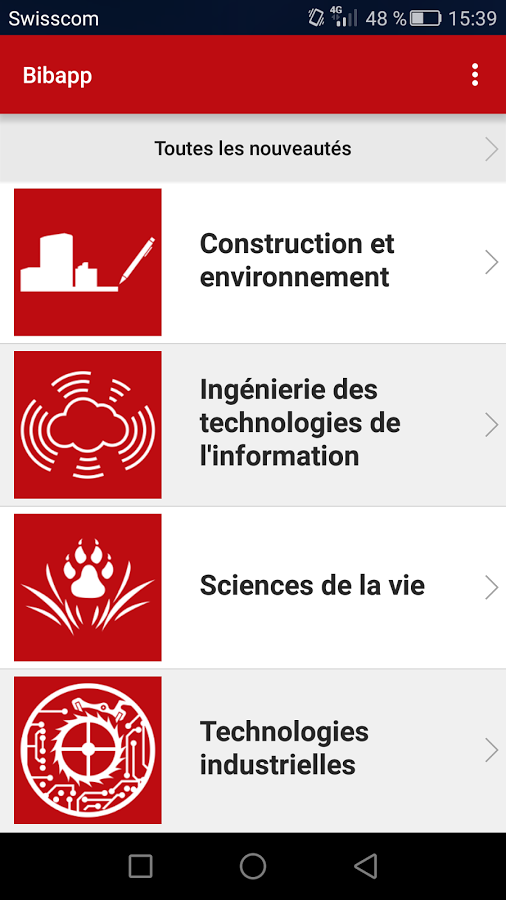
\includegraphics[width=1\textwidth]{images/bibapp.png}
                    \end{figure}
                \end{column}
                \begin{column}{.3\textwidth}
                    \begin{figure}
                        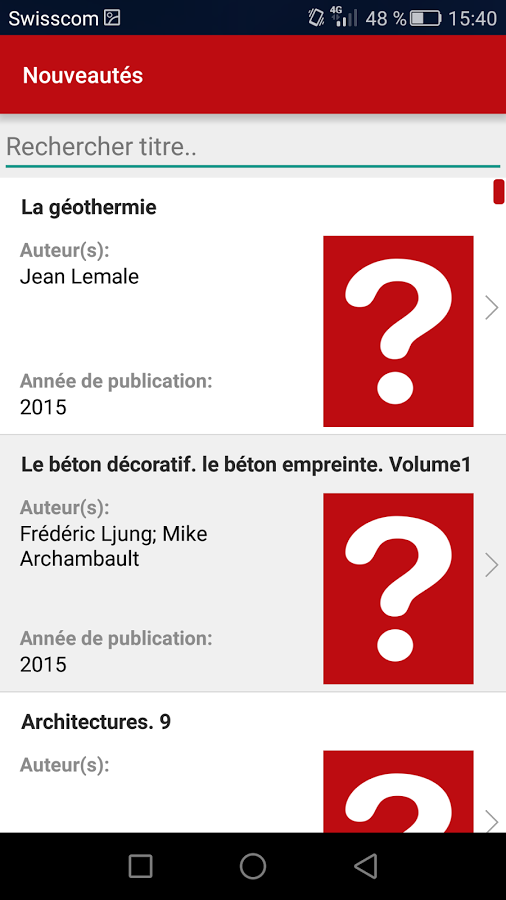
\includegraphics[width=1\textwidth]{images/bibapp2.png}
                    \end{figure}
                \end{column}
                \begin{column}{.3\textwidth}
                    \begin{figure}
                        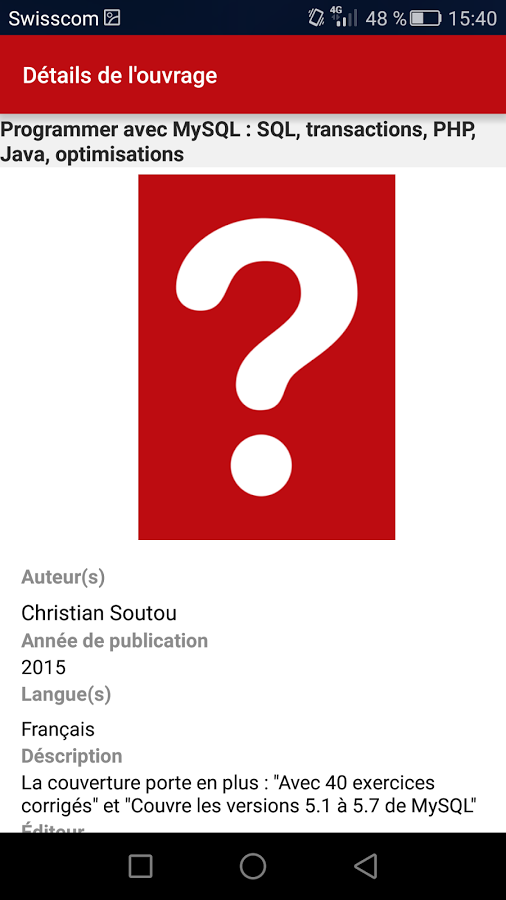
\includegraphics[width=1\textwidth]{images/bibapp3.png}
                    \end{figure}
                \end{column}
            \end{columns}
		\end{column}
		\begin{column}{.35\textwidth}
			\begin{itemize}
				\item Nouveautés listées par section
                \item Affiche les détails du livre
                \item Android et iOS
                \item Par Cicciù et Minelli
			\end{itemize}
		\end{column}
	\end{columns}
\end{frame}

\subsection{Objectifs}
\begin{frame}
	\frametitle{\secname}
	\framesubtitle{\subsecname}
    \begin{itemize}
        \item Étude du framework Ionic (tuto + prototype)
        \item Architecture de l'application mobile/web (backend, frontend et interfaces)
        \item Réalisation de la base de données augmentée
        \begin{itemize}
            \item Basée sur les données de NEBIS
            \item Enrichie avec les données saisies par la bibliothèque
            \item Accessible via API REST avec mode client et administrateur
        \end{itemize}
        \item Design et implémentation des interfaces en collaboration avec la bibliothèque
        \begin{itemize}
            \item Tests unitaires
            \item Échanges avec les bibliothécaires
        \end{itemize}
    \end{itemize}
\end{frame}

\section{Situation actuelle}
\begin{frame}
	\frametitle{\secname}
    \begin{itemize}
        \item Étude du framework Ionic et écosystème (Angular, Typescript)
        \item Reprise/amélioration de BibApp V1 avec Ionic
        \item Élaboration de l'architecture
        \item Accès à l'API NEBIS (tout récent)
    \end{itemize}
\end{frame}

\section{Planification}
\subsection{Prochains mois/semaines}
\begin{frame}
	\frametitle{\secname}
	\framesubtitle{\subsecname}
	\begin{itemize}
        \item Améliorer l'application Ionic
        \item Rencontres/échanges avec la bibliothèque
        \item Étudier l'API NEBIS
        \item Réalisation du backend et de la base de données
    \end{itemize}
\end{frame}

\subsection{Architecture}
\begin{frame}
	\frametitle{\secname}
	\framesubtitle{\subsecname (1)}
	\begin{figure}
		\begin{center}
			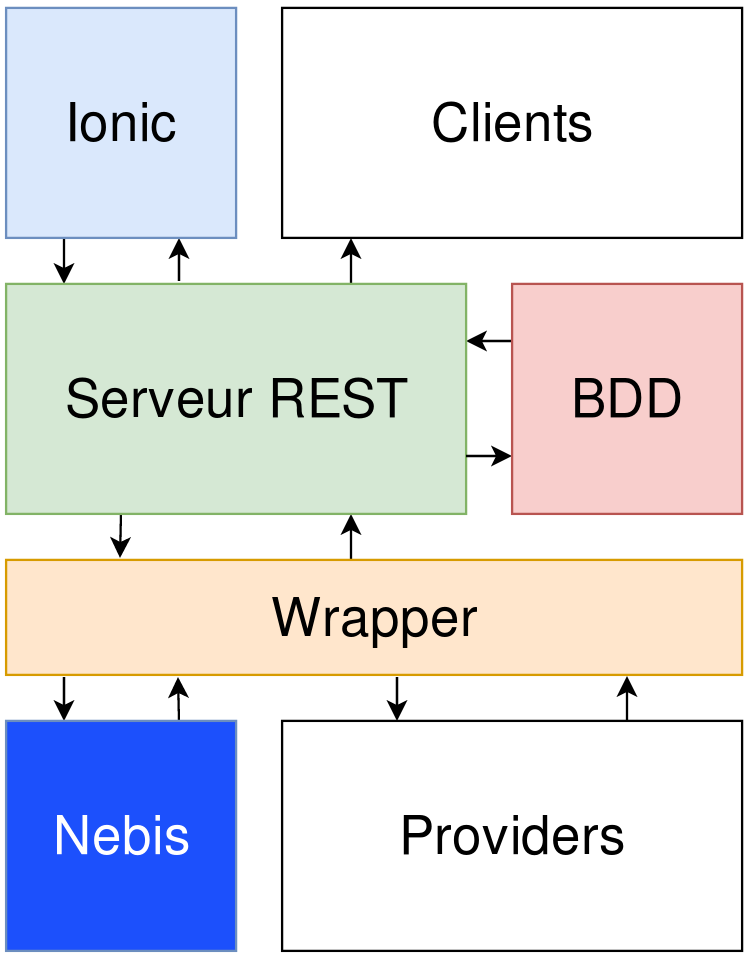
\includegraphics[width=0.5\textwidth]{images/architecture.png}
		\end{center}
	\end{figure}
\end{frame}

\begin{frame}
	\frametitle{\secname}
	\framesubtitle{\subsecname (2)}
	\begin{figure}
		\begin{center}
			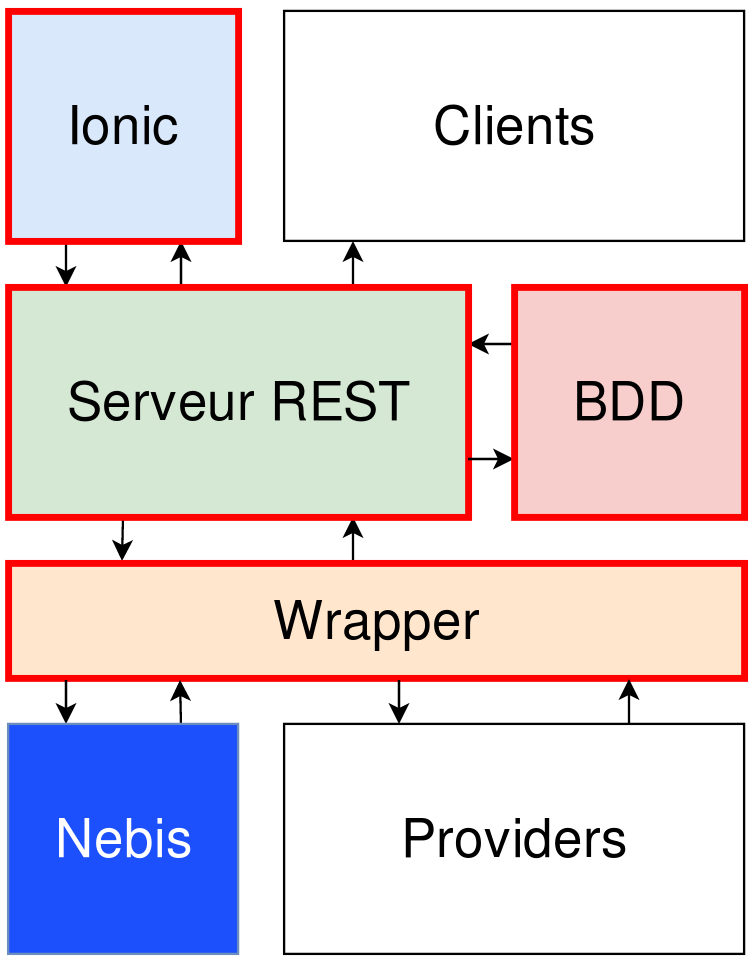
\includegraphics[width=0.5\textwidth]{images/architecture2.png}
		\end{center}
	\end{figure}
\end{frame}

\end{document}
